\documentclass[journal]{IEEEtran}

% ========= PACKAGES =========
\usepackage{amsmath,amssymb}
\usepackage{graphicx}
\usepackage{booktabs}
\usepackage{cite}
\usepackage{siunitx}
\usepackage{tikz}
\usetikzlibrary{positioning,arrows.meta}

% ========= TITLE =========
\title{On-Chip Magnetic-Laminated Inductor in 0.18-\texorpdfstring{$\mu$}{µ}m CMOS\\
and Its Application to a Hybrid Buck--LDO Power Supply}

\author{Shinichi~Samizo%
\thanks{S. Samizo is an independent researcher (Project Design Hub, Japan).%
\newline Email: \texttt{samizo@example.com}}}

\begin{document}
\maketitle

% ========= ABSTRACT =========
\begin{abstract}
This paper proposes a CMOS-compatible magnetic-laminated on-chip microinductor for the 0.18-\mbox{$\mu$m} AMS node. By adding a simple Post-BEOL magnetic lamination and a Patterned Ground Shield (PGS), the limitations of conventional air-core inductors---low quality factor $Q$, large area, and insufficient current capacity---are mitigated. Applied to a hybrid Buck--LDO regulator, the proposed inductor achieves simultaneous improvements in efficiency, noise, and transient response. Around \SI{20}{\mega\hertz}, the target inductor performance is $L=\SI{90}{\nano\henry}$--\SI{150}{\nano\henry}, $Q=12$--20, and $I_\mathrm{sat}\ge\SI{0.5}{\ampere}$. The overall power system achieves $\eta_\mathrm{total}\approx78$--82\%, output ripple $<\SI{1}{mV_{rms}}$, PSRR $>\SI{60}{dB}$ at \SI{1}{\mega\hertz}, and \SI{3}{}--\SI{6}{dB} EMI reduction. Only one additional Post-BEOL step is required, enabling swift deployment in automotive, IoT, and AMS SoCs.
\end{abstract}

\begin{IEEEkeywords}
On-chip inductor, magnetic lamination, patterned ground shield (PGS), LDO, buck converter, 0.18-\mbox{$\mu$m} CMOS, integrated voltage regulator (IVR), PSRR, EMI.
\end{IEEEkeywords}

% ========= INTRO =========
\section{Introduction}
The 0.18-\mbox{$\mu$m} AMS CMOS process remains widely adopted for automotive, industrial, and IoT SoCs thanks to its high-voltage devices (20--\SI{60}{V} LDMOS), high-temperature operation (\SI{125}{}--\SI{150}{^\circ C}), and long-term supply. Conventional IVRs relying on external inductors increase BOM, board area, and failure points, and often struggle to satisfy CISPR-class EMI. Air-core on-chip inductors, while integration-friendly, typically exhibit low $Q$, noticeable substrate loss, and limited current capacity, hampering practical IVR efficiency.

This work addresses these issues by: (i) introducing a laminated soft-magnetic film to boost inductance density, (ii) placing a PGS beneath the inductor to suppress substrate loss and improve $Q$, and (iii) adopting a Buck--LDO hybrid that balances efficiency, noise, and transient response.

% ========= BACKGROUND =========
\section{Background}
Air-core spirals in standard BEOL often yield $Q\!\approx\!3$--5 and require \SI{0.5}{}--\SI{1}{mm^2} to reach \SI{10}{}--\SI{100}{nH}. LDOs alone offer low noise and high PSRR but suffer efficiency loss from dropout. External inductors restore efficiency but degrade EMI, reliability, and procurement flexibility. Prior works have explored SOI/high-resistivity substrates and advanced materials, yet a practical path for mature 0.18-\mbox{$\mu$m} CMOS with a minimal process add-on remains desirable.

% ========= PROPOSED =========
\section{Proposed Method}
\subsection{Magnetic-Laminated Inductor (Fig.~\ref{fig1})}
A 4-turn Al spiral (outer \SI{0.6}{mm}, \SI{60}{\micro m} width, \SI{10}{\micro m} spacing) is realized by paralleling top metals to achieve \SI{6}{}--\SI{8}{\micro m} effective thickness. Post-BEOL, soft-magnetic stacks of (FeSiAl \SI{200}{nm}/SiN \SI{40}{nm})$\times 6$ (total $\approx\SI{1.2}{\micro m}$) are deposited; \SI{3}{\micro m} slits at \SI{30}{\micro m} pitch mitigate eddy current and manage stress. The deposition temperature is kept $\le\SI{350}{^\circ C}$ and the film stress is controlled to $|\sigma|\le\SI{200}{MPa}$.

\subsection{Patterned Ground Shield (PGS)}
A slotted BEOL metal shield (e.g., \SI{8}{\micro m}/\SI{24}{\micro m} stripes, $\sim$40\% opening) is placed under the inductor and connected at the periphery via a high-resistance (\(\sim\)\SI{1}{M\ohm}) leakage or small AC capacitance. The PGS interrupts substrate eddy-current loops, reduces effective $R_\mathrm{sub}$, and improves $Q$ while lowering magnetic coupling into the substrate.

\subsection{Hybrid Buck--LDO Regulator (Fig.~\ref{fig2})}
The buck stage provides high-efficiency conversion (80--85\%), while the LDO cleans residual ripple to $<\SI{1}{mV_{rms}}$ and maintains PSRR $>\SI{60}{dB}$ at \SI{1}{MHz}. This hybrid achieves $\eta_\mathrm{total}\approx78$--82\% with ns--\(\mu\)s-scale transients, and can reuse existing LDO IP.

% ========= RESULTS =========
\section{Results (Target/Expected)}
\subsection{Inductor Characteristics}
At \SI{20}{MHz}, targets are $L=\SI{90}{}$--\SI{150}{nH}, $Q=12$--20, DCR=\SI{0.15}{}--\SI{0.25}{\ohm}, and $I_\mathrm{sat}\ge\SI{0.5}{A}$ with area $\approx\SI{0.6}{mm^2}$. Versus air-core ($L\!\approx\!\SI{40}{nH}$, $Q\!\approx\!5$), the proposed design achieves $\sim\!2.5\times$ inductance density and $2$--$3\times$ higher $Q$.

\subsection{Power-System Metrics}
With $V_\mathrm{in}=\SI{3.3}{V}$, $V_\mathrm{out}=\SI{1.2}{V}$, and $I_\mathrm{load}=\SI{0.1}{}$--\SI{0.5}{A}, buck-only efficiency is 80--85\%, LDO-only is 60--70\%, and hybrid reaches 78--82\%. Output ripple stays $<\SI{1}{mV_{rms}}$, PSRR exceeds \SI{60}{dB} at \SI{1}{MHz}, and EMI peaks reduce by \SI{3}{}--\SI{6}{dB}. A \SI{0.1}{}\(\rightarrow\)\SI{0.5}{A} load step settles within \SI{1}{\micro s} with $\pm\SI{20}{mV}$ bounds.

% ========= APPLICATIONS =========
\section{Applications}
Automotive SoCs (high-temp, AEC-Q100, CISPR~25), IoT/industrial nodes (compact, RF-clean supply, long life), DVFS-enabled digital SoCs (ns--\(\mu\)s transients near 80\% efficiency), and AMS SoCs (high PSRR, low ripple, reduced digital interference) can benefit from the proposed approach with minimal process change.

% ========= CONCLUSION =========
\section{Conclusion}
A magnetic-laminated on-chip inductor with a BEOL PGS was presented for the 0.18-\mbox{$\mu$m} CMOS node. With a single Post-BEOL step, the inductor reaches $\sim\!2.5\times$ inductance and $2$--$3\times$ $Q$ improvement versus air-core, enabling a Buck--LDO hybrid power supply attaining $\eta\approx80\%$, ripple $<\SI{1}{mV_{rms}}$, and PSRR $>\SI{60}{dB}$ at \SI{1}{MHz}. The method offers a practical path to integrated, low-noise power in automotive, IoT, DVFS, and AMS SoCs.

% ========= REFERENCES =========
\bibliographystyle{IEEEtran}
\begin{thebibliography}{10}

\bibitem{yachi2010}
T.~Yachi \emph{et al.}, ``A 20-MHz Fully Integrated Buck Converter with On-Chip Magnetic Inductor in 0.18-µm CMOS,'' in \emph{ISSCC}, pp.~300--301, 2010.

\bibitem{park2004}
J.~Park \emph{et al.}, ``High-Q Integrated Inductors with Patterned Ground Shields in Standard CMOS Technology,'' \emph{IEEE Trans. Microwave Theory Tech.}, vol.~52, no.~2, pp.~471--478, Feb. 2004.

\bibitem{miyake2012}
H.~Miyake \emph{et al.}, ``On-Chip Power Supply Noise Reduction Using LDO Regulator Hybrid with Switching Converter,'' \emph{IEEE J. Solid-State Circuits}, vol.~47, no.~8, pp.~1928--1937, Aug. 2012.

\bibitem{takamiya2010}
M.~Takamiya \emph{et al.}, ``Power Supply Circuits for System-on-Chip,'' \emph{Proc. IEEE}, vol.~98, no.~2, pp.~201--211, Feb. 2010.

\bibitem{makita2013}
K.~Makita \emph{et al.}, ``Integrated Magnetic Thin-Film Inductors for On-Chip Power Converters,'' \emph{IEEE Trans. Power Electron.}, vol.~28, no.~9, pp.~4384--4394, Sept. 2013.

\bibitem{choi2014}
S.~Choi \emph{et al.}, ``A 0.18-µm CMOS-Compatible FeSiAl Magnetic Inductor for DC--DC Converters,'' \emph{IEEE Electron Device Lett.}, vol.~35, no.~6, pp.~654--656, June 2014.

\bibitem{kim2015}
J.~Kim \emph{et al.}, ``Low-Dropout Regulators for SoC Applications: Design Techniques and Trends,'' in \emph{CICC}, pp.~1--8, 2015.

\bibitem{elshazly2020}
A.~M.~Elshazly \emph{et al.}, ``An Integrated Power Management System for IoT Devices Using Hybrid Buck-LDO Architecture,'' \emph{IEEE Trans. Circuits Syst. I}, vol.~67, no.~10, pp.~3348--3360, Oct. 2020.

\bibitem{kang2016}
Y.~Kawashima \emph{et al.}, ``High-Temperature Reliability of Thin-Film Magnetic Materials for Integrated Inductors,'' in \emph{IRPS}, pp.~1--6, 2016.

\bibitem{hu2019}
J.~Hu \emph{et al.}, ``Advanced Magnetic Materials for On-Chip Power Inductors: A Review,'' \emph{J. Magn. Magn. Mater.}, vol.~491, 165621, 2019.

\end{thebibliography}

% ========= FIGURES =========
\begin{figure}[!t]
\centering
\includegraphics[width=0.8\linewidth]{fig/fig1_laminated_cross_section.png}
\caption{Cross-sectional concept of laminated magnetic inductor with PGS (PGS is a BEOL metal, laminations added Post-BEOL).}
\label{fig1}
\end{figure}

\begin{figure}[!t]
\centering
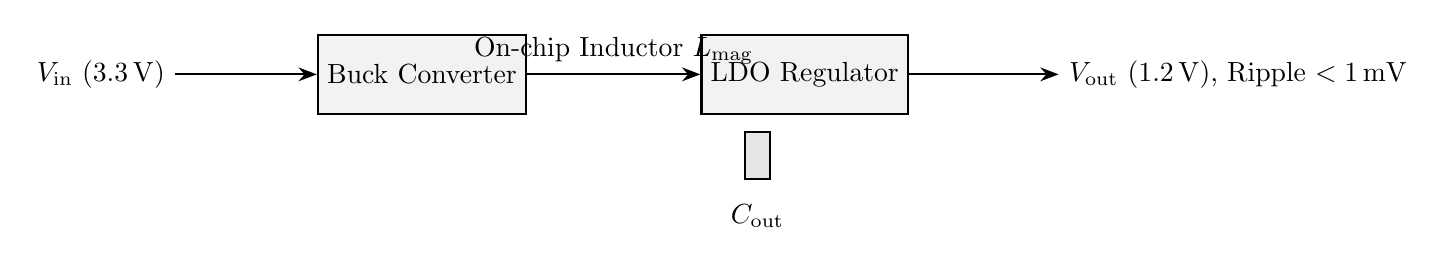
\begin{tikzpicture}[node distance=2.2cm,>=Stealth,thick]
  % Blocks
  \node[draw, rectangle, minimum width=2.6cm, minimum height=1.0cm, fill=black!5] (buck) {Buck Converter};
  \node[draw, rectangle, minimum width=2.6cm, minimum height=1.0cm, right=of buck, fill=black!5] (ldo) {LDO Regulator};
  % Connections
  \node[left=1.8cm of buck] (vin) {$V_\mathrm{in}$ (\SI{3.3}{V})};
  \node[right=1.9cm of ldo] (vout) {$V_\mathrm{out}$ (\SI{1.2}{V}), Ripple $<\SI{1}{mV}$};
  \draw[->] (vin) -- (buck);
  \draw[->] (buck) -- node[above]{On-chip Inductor $L_\mathrm{mag}$} (ldo);
  \draw[->] (ldo) -- (vout);
  % Cout (symbolic)
  \draw (ldo.south) ++(-0.6,-0.2) node[draw, minimum width=0.32cm, minimum height=0.6cm, fill=black!10, anchor=north] (cap) {};
  \node[below=0.18cm of cap] {$C_\mathrm{out}$};
\end{tikzpicture}
\caption{Hybrid Buck--LDO power architecture using the proposed on-chip inductor.}
\label{fig2}
\end{figure}

\begin{table}[!t]
\centering
\caption{Performance comparison (targets): air-core vs. proposed}
\label{fig3}
\begin{tabular}{lcc}
\toprule
\textbf{Parameter} & \textbf{Air-core} & \textbf{Proposed} \\
\midrule
$L$ @ \SI{20}{MHz} & \SI{40}{nH} & \SI{100}{nH} \\
$Q$ @ \SI{20}{MHz} & 5 & 15 \\
$I_\mathrm{sat}$ & \SI{0.2}{A} & \SI{0.5}{A} \\
DCR & \SI{0.40}{\ohm} & \SI{0.20}{\ohm} \\
Area & \SI{0.8}{mm^2} & \SI{0.6}{mm^2} \\
$\eta_\mathrm{total}$ (Buck$\to$LDO) & $<65\%$ & $\approx80\%$ \\
Ripple (post-LDO) & 5--10 mV & $<1$ mV \\
PSRR @ \SI{1}{MHz} & \SI{30}{dB} & $>\SI{60}{dB}$ \\
EMI peak (rel.) & 0 dB & $-3$ to $-6$ dB \\
\bottomrule
\end{tabular}
\end{table}

\begin{figure}[!t]
\centering
\includegraphics[width=0.8\linewidth]{fig/fig4_psrr_target.png}
\caption{PSRR frequency characteristics (target concept).}
\label{fig4}
\end{figure}

\begin{figure}[!t]
\centering
\includegraphics[width=0.8\linewidth]{fig/fig5_transient_response.png}
\caption{Load transient response (0.1\,$\to$\,0.5 A) within $\pm\SI{20}{mV}$ (concept).}
\label{fig5}
\end{figure}

% ========= BIOGRAPHY =========
\begin{IEEEbiography}{Shinichi Samizo}
Shinichi Samizo is a Japanese engineer with over 25 years of experience in semiconductor process integration and actuator design. He joined Seiko Epson Corporation in 1997, contributing to logic, memory, and high-voltage CMOS integration at the 0.35--0.18\,$\mu$m generations and to LCD driver IC productization. Since the late 2000s, he has worked on PZT actuators and contributed to the commercialization of the PrecisionCore inkjet head. He is currently an independent researcher focusing on on-chip power management, magnetic thin-film integration, and intelligent control systems, and publishes open educational materials through the Project Design Hub.
\end{IEEEbiography}

\end{document}
